\chapter{Dostępne rozwiązania}
\label{sec:dostepnerozwiazania}

Przed rozpoczęciem implementacji własnego rozwiązania postanowiono przeprowadzić badania mające na celu analizę aktualnie dostępnych rozwiązań spełniających przynajmniej w części założenia. Proces ten nie ma na celu znalezienie idealnego rozwiazania lecz poznanie różnych podejść do zagadnienia, analiza różnych technologi które mogą być wykorzytane pozwoli na świadome wybranie najlepszych.


\section{Google Earth}
\label{sec:Google Earth}

Funkcjonalnośc interaktywnych map można znaleść w aplikacji stworzonej przez firmę Google. Program ten jest napisany przy użyciu języka C++, nie służy on do tworznia aplikacji mobilnych, dlatego nie został on wybrany jako kandydat do naszej pracy.

Wykorzystuje ono statyczne obrazy będące zdjęciami satelitarnymi dla obrazów w dużej wysokośći lub zdjęciami wykonanymi z pokładów samolotów. Pomimo duzej atrakcyjności ma ono bardzo ograniczoną możliwośći zmiany oglądanych danych, ograniczone do ilości wykonanych zdjęć, dodatkowo większość punktów najstarsze dane ma z lat 50 XX w.

Przykład takiej sytuacji został przedstawiony na rysunku \ref{fig:lasVegas1}, obraz terenu na którym powstanie miasto Las Vegas w roku 1950. Jak teren ten wyglądał w roku 1977 widzimy na rysunku \ref{fig:lasVegas2}, pomimo widocznych zmian teren ten nadal w dużym stopniu jest pustynny,dopiero na rysunku \ref{fig:lasVegas3} widzimy aktualny stan miasta.

Dzięki funkcji zmiany punktu i kąta patrzenia, pokazywania ciekawych miejsc czy chociażby włączania trybu w którym budynki nabierają formy przestrzennej, 3D, możemy poprzez zabawę i wirtualne wycieczki poszeżać naszą wiedzę o otaczającym nas świecie.


\begin{figure}[H]
  \centering
    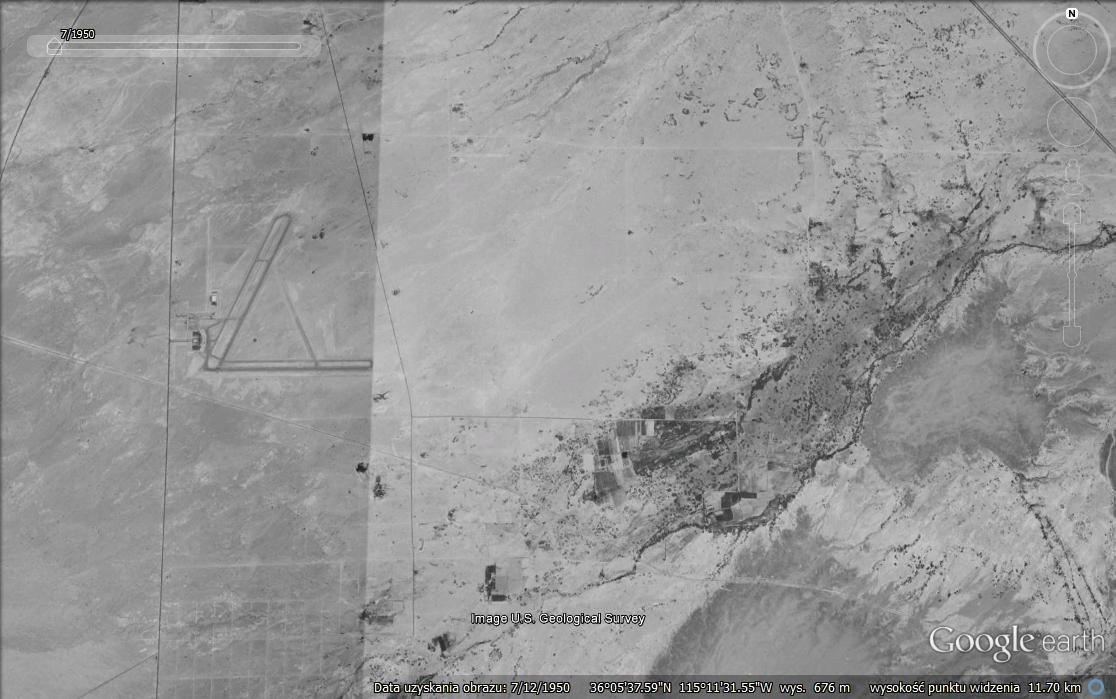
\includegraphics[width=100mm]{ge/01_1950.jpg}
  \caption{Las Vegas w 1950 roku.}
  \label{fig:lasVegas1}
\end{figure}

\begin{figure}[H]
  \centering
    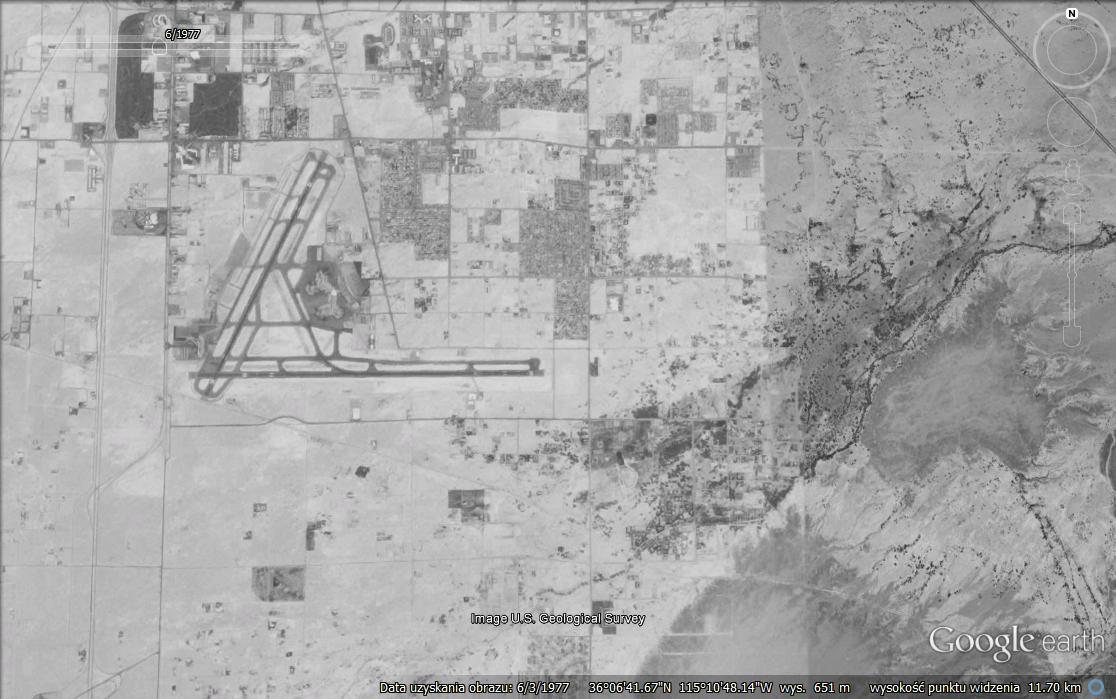
\includegraphics[width=100mm]{ge/02_1977.jpg}
  \caption{Las Vegas w 1950 roku.}
  \label{fig:lasVegas2}
\end{figure}

\begin{figure}[H]
  \centering
    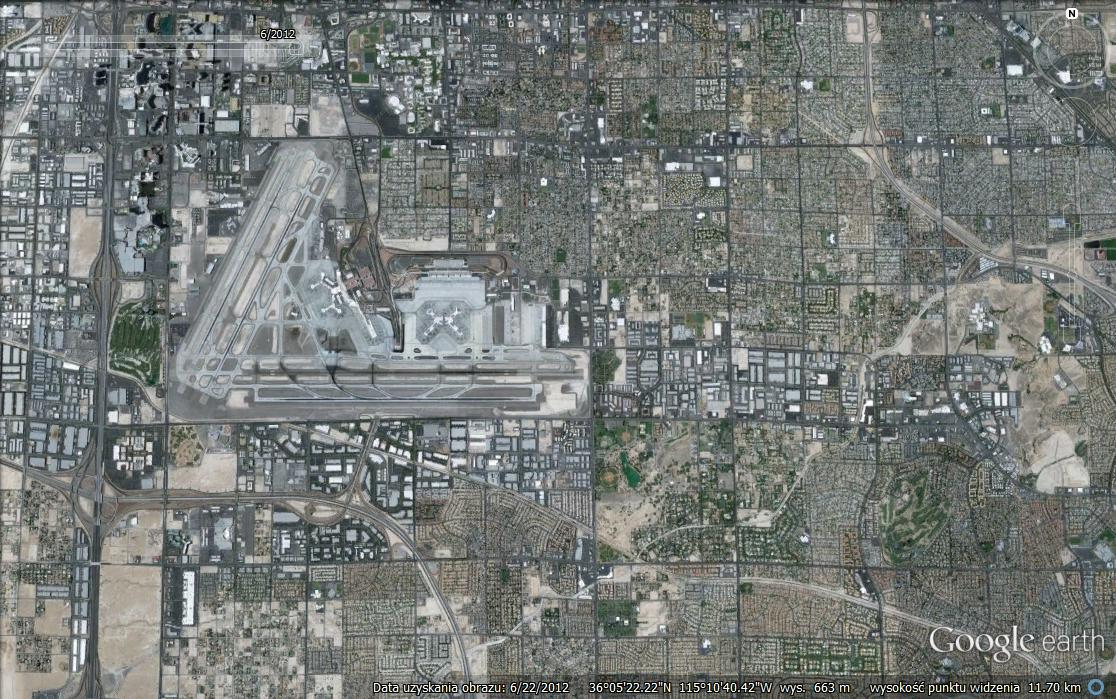
\includegraphics[width=100mm]{ge/03_2012.jpg}
  \caption{Las Vegas w 1950 roku.}
  \label{fig:lasVegas3}
\end{figure}

\section{Aplikacje wykonane w technologi Flash}
\label{sec:flashmap}

Podczas prac badawczych natrafiono na kilka aplikacji któych główna część aplikcji została wykonana w technologi flash. Przykładami są interaktywna mapa historii europy \cite{worldology}, mapa prezentująca zmianę granic państw w XX wieku \cite{flashborder}. Oba przykłady zawierają bogatą szatę graficzną, ich wykonanie jest bardzo estetyczne.

Niewąpliwą wadę aplikacji wykonanych w tej technologi jest utrudniony proces wprowadzania zmian. Ze względu na obecność pliku wykonywalnego wymagane jest korzystanie ze specjalnych narzędzi.

\section{Wybrane technologie}
\label{sec:technologie}